\documentclass{article}
\usepackage{amsfonts, amsthm, amsmath, amssymb, mathtools, ulem, mathrsfs, physics, esint, siunitx, tikz-cd}
\usepackage{pdfpages, fullpage, color, microtype, cancel, textcomp, markdown, hyperref, graphicx}
\usepackage{enumitem}
\graphicspath{{./images/}}
\usepackage[english]{babel}
\usepackage[autostyle, english=american]{csquotes}
\MakeOuterQuote{"}
\usepackage{xparse}
\usepackage{tikz}
\usepackage{algpseudocode}

% fonts
\def\mbb#1{\mathbb{#1}}
\def\mfk#1{\mathfrak{#1}}
\def\mbf#1{\mathbf{#1}}
\def\tbf#1{\textbf{#1}}

% common bold letters
\def\bP{\mbb{P}}
\def\bC{\mbb{C}}
\def\bH{\mbb{H}}
\def\bI{\mbb{I}}
\def\bR{\mbb{R}}
\def\bQ{\mbb{Q}}
\def\bZ{\mbb{Z}}
\def\bN{\mbb{N}}

% brackets
\newcommand{\br}[1]{\left(#1\right)}
\newcommand{\sbr}[1]{\left[#1\right]}
\newcommand{\brc}[1]{\left\{#1\right\}}
\newcommand{\lbr}[1]{\left\langle#1\right\rangle}

% matrices
\newcommand{\m}[2][b]{\begin{#1matrix}#2\end{#1matrix}}
\newcommand{\arr}[3][\sbr]{#1{\begin{array}{#2}#3\end{array}}}
\DeclareMathOperator{\Span}{span}

% greek
\newcommand{\e}{\epsilon}
\newcommand{\p}{\varphi}
\renewcommand{\t}{\theta}
\renewcommand{\S}{\Sigma}
\newcommand{\s}{\sigma}

% misc
\NewDocumentCommand{\app}{O{x} O{\infty}}{\xrightarrow{#1\to#2}}
\newcommand{\sse}{\subseteq}
\renewcommand{\ss}{\subset}
\newcommand{\vn}{\varnothing}
\newcommand{\inv}{^{-1}}
\newcommand{\imp}{\implies}
\newcommand{\impleft}{\reflectbox{$\implies$}}
\renewcommand{\ip}[2]{\lbr{#1,#2}}
\renewcommand{\bar}{\overline}
\DeclareMathOperator{\cis}{cis}
\DeclareMathOperator{\Arg}{Arg}
\renewcommand{\d}{\partial}
\newcommand{\pf}{\tbf{Proof. }}
\renewcommand{\L}{\mathcal{L}}

% title
\title{Scientific Computing HW 6}
\author{Ryan Chen}
%\date{\today}
\setlength{\parindent}{0pt}


\begin{document}
	
\maketitle



Note: For sums we assume the lower bound to be 1 unless otherwise specified, and we will not specify upper bounds since they are determined by the sizes of our matrices.

\begin{enumerate}
	
	
	
	\item 
	
	\begin{enumerate}
		
		
		
		\item Consider the following.
		\[\sum_i\sum_j\sum_k a_{ik}b_{kj}c_{ji} = \sum_i\sum_j\sum_k b_{kj}c_{ji}a_{ik} = \sum_i\sum_j\sum_k c_{ji}a_{ik}b_{kj}\]
		The first, second, and third expressions are, respectively, $\tr(ABC)$, $\tr(BCA)$, and $\tr(CAB)$.
		
		
		
		\item Compute
		\begin{align*}
			\norm{A}_F^2 &= \sum_i\sum_j a_{ij}^2 \\
			&= \tr(A^TA) \\
			&= \tr(V\S U^TU\S V^T) & A = U\S V^T \\
			&= \tr(V\S^2V^T) \\
			&= \tr(\S^2V^TV) & \text{cyclic property of trace} \\
			&= \tr(\S^2) \\
			&= \sum_i \s_i^2
		\end{align*}
		
		
		
		\item Compute
		\begin{align*}
			\norm{A+B}_F^2 &= \sum_i\sum_j (a_{ij}+b_{ij})^2 \\
			&= \sum_i\sum_j a_{ij}^2 + \sum_i\sum_j b_{ij}^2 + 2\sum_i\sum_j a_{ij}b_{ij} \\
			&= \norm{A}_F^2 + \norm{B}_F^2 + 2\ip{A}{B}_F
		\end{align*}
		
		
		
	\end{enumerate}



	\pagebreak
	
	
	
	\item Observe that
	\[A_k = U_k\S_kV_k^T = U\S_k'V^T\]
	where $\S_k'$ is obtained by adding zeros to $\S_k$ to make it the same size as $\S$. Then
	\[A - A_k = U(\S-\S_k')V^T\]
	is an SVD of $A-A_k$ with the $j$th diagonal entry of $\S-\S_k'$ being 0 for $j\le k$ and $\s_j(A)$ for $j>k$. Denoting the Ky Fan $p-$norm by $\norm{\cdot}_{KF(p)}$,
	\[\norm{A-A_k}_{KF(p)}^p = \sum_j \s_j^p(A-A_k) = \sum_{j\ge k+1} \s_j^p(A)\]
	Fix a matrix $M$ with $\rank M\le k$. By Lemma 1 in Section 4.3 of the lecture notes,
	\[\s_{k+i}(A) \le \s_i(A-M) + \s_{k+1}(M) = \s_i(A-M)\]
	Then we have
	\begin{align*}
		\norm{A-M}_{KF(p)}^p &= \sum_i \s_i^p(A-M) \\
		&\ge \sum_i \s_{k+i}^p(A) & \s_{k+i}(A) \le \s_i(A-M) \\
		&= \sum_{j\ge k+1} \s_j^p(A) & \text{change variables } j := k+i \\
		&= \norm{A-A_k}_{KF(p)}^p
	\end{align*}
	Taking the $p$th root of both sides gives $\norm{A-M}_{KF(p)} \ge \norm{A-A_k}_{KF(p)}$.



	\pagebreak
	
	
	
	\item Code: \url{https://github.com/RokettoJanpu/scientific-computing-1-redux/blob/main/hw6.ipynb}
	
	\begin{enumerate}
		
		
		
		\item Here we run PGD five times.
		\begin{center}
			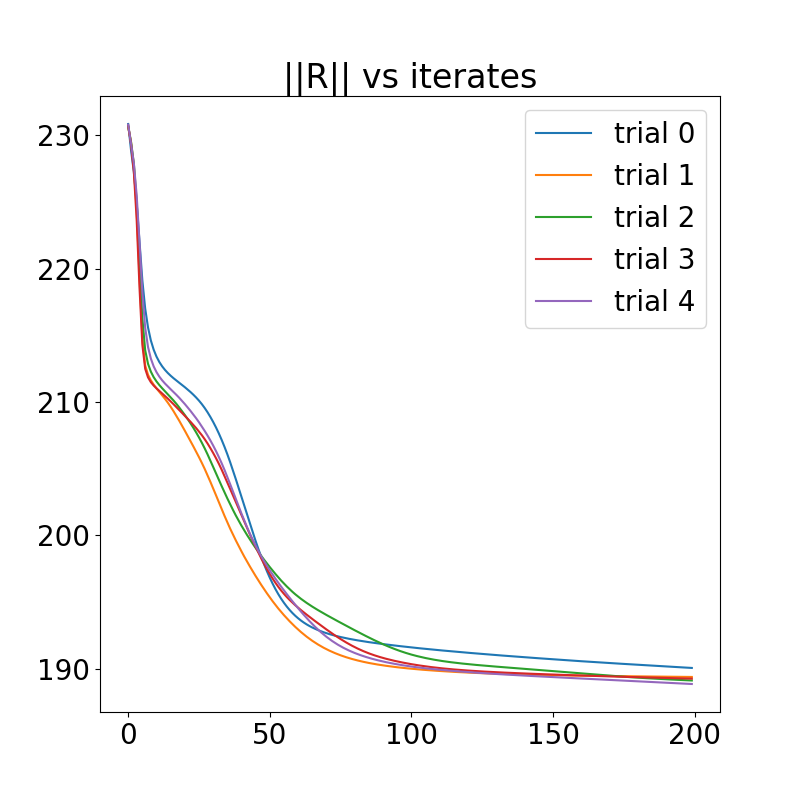
\includegraphics[scale=.3]{hw6 pgd}
		\end{center}
		The residual norm settles at around 80 iterations. Its eventual value is about 190 in each trial. Examining entries of $W$ greater than 0.2, we hypothesize that the documents are advertizements of events and services in various communities across the country.
		
		
		
		\item Here we run HALS five times.
		\begin{center}
			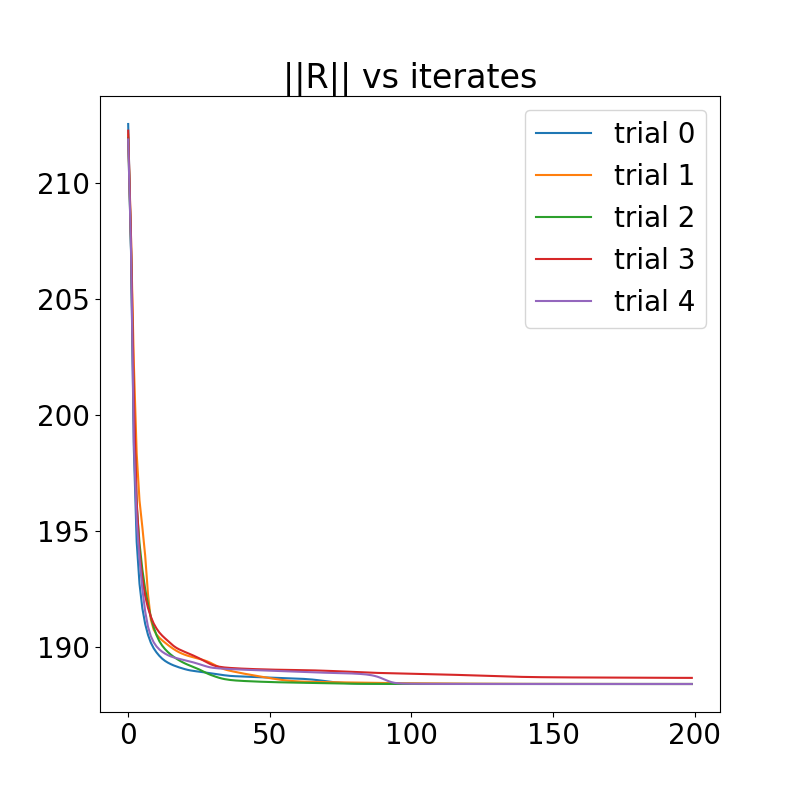
\includegraphics[scale=.3]{hw6 hals}
		\end{center}
		The residual norm settles at around 20 iterations. Its eventual value is about 188 in each trial. 
		

		
		\item Using the SVD of $A$, we find $\norm{A-A_{10}}_F\approx 187.72$, slightly below the residual norms of both PGD and HALS, as expected by the Eckart--Young--Mirsky theorem.
		
		
		
	\end{enumerate}
	
	
	
\end{enumerate}

	
	
\end{document}